%%%%%%%%%%%%%%%%%%%%%%%%%%%%%%%%%%%%%%%%%
% Beamer Presentation
% LaTeX Template
% Version 1.0 (10/11/12)
%
% This template has been downloaded from:
% http://www.LaTeXTemplates.com
%
% License:
% CC BY-NC-SA 3.0 (http://creativecommons.org/licenses/by-nc-sa/3.0/)
%
%%%%%%%%%%%%%%%%%%%%%%%%%%%%%%%%%%%%%%%%%

%----------------------------------------------------------------------------------------
%	PACKAGES AND THEMES
%----------------------------------------------------------------------------------------

\documentclass{beamer} 
%\usepackage[font=small,skip=0pt]{caption}
\setbeamertemplate{caption}[numbered]
%\captionsetup[figure]{font=small,skip=0pt}
\mode<presentation> {

% The Beamer class comes with a number of default slide themes
% which change the colors and layouts of slides. Below this is a list
% of all the themes, uncomment each in turn to see what they look like.

%\usetheme{default}
%\usetheme{AnnArbor}
%\usetheme{Antibes}
%\usetheme{Bergen}
%\usetheme{Berkeley}
%\usetheme{Berlin}
%\usetheme{Boadilla}
%\usetheme{CambridgeUS}
%\usetheme{Copenhagen}
%\usetheme{Darmstadt}
%\usetheme{Dresden}
%\usetheme{Frankfurt}
%\usetheme{Goettingen}
%\usetheme{Hannover}
%\usetheme{Ilmenau}
%\usetheme{JuanLesPins}
%\usetheme{Luebeck}
\usetheme{Madrid}
%\usetheme{Malmoe}
%\usetheme{Marburg}
%\usetheme{Montpellier}
%\usetheme{PaloAlto}
%\usetheme{Pittsburgh}
%\usetheme{Rochester}
%\usetheme{Singapore}
%\usetheme{Szeged}
%\usetheme{Warsaw}

% As well as themes, the Beamer class has a number of color themes
% for any slide theme. Uncomment each of these in turn to see how it
% changes the colors of your current slide theme.

%\usecolortheme{albatross}
%\usecolortheme{beaver}
%\usecolortheme{beetle}
%\usecolortheme{crane}
%\usecolortheme{dolphin}
%\usecolortheme{dove}
%\usecolortheme{fly}
%\usecolortheme{lily}
%\usecolortheme{orchid}
%\usecolortheme{rose}
%\usecolortheme{seagull}
%\usecolortheme{seahorse}
%\usecolortheme{whale}
%\usecolortheme{wolverine}

%\setbeamertemplate{footline} % To remove the footer line in all slides uncomment this line
%\setbeamertemplate{footline}[page number] % To replace the footer line in all slides with a simple slide count uncomment this line

%\setbeamertemplate{navigation symbols}{} % To remove the navigation symbols from the bottom of all slides uncomment this line
}
\graphicspath{{Figures/}}
\usepackage{graphicx} % Allows including images
\usepackage{booktabs} % Allows the use of \toprule, \midrule and \bottomrule in tables
\usepackage[ruled,boxed]{algorithm2e}
\newcommand{\HRule}{\rule{\linewidth}{0.5mm}} % New command to make the lines in the title page
%\newtheorem{lemma}{Lemma}
% \newtheorem{thm}{Theorem}
\newtheorem{thm}{{\break \noindent {\bf Theorem}}}

\newcommand{\loc}   	{ {\mathrm {Loc}} }
\newcommand{\ACONN}   { {\mathrm {A\mbox{-}CONN}} }
\newcommand{\SCONN}   { {\mathrm {S\mbox{-}CONN}} }
\newcommand{\ARCONN}   { {\mathrm {AR\mbox{-}CONN}} }
\newcommand{\SRCONN}   { {\mathrm {SR\mbox{-}CONN}} }
\newcommand{\GV}   { {\mathrm {G=(V,E_G,Loc,p)} }}

\newcommand{\fConn}   	{ {\mathrm {Conn}} }

\newcommand{\nReq}    { {n_{req}} }
\newcommand{\boldS}   { \mathbf{S}}
\newcommand{\DCH}     { {DCH} }

%% -- older paper --

\newcommand{\starEqual}   { {\;{\scriptstyle *} \! =} }
\newcommand{\plusEqual}   { {\;{\scriptstyle +} \! =} }
%\newcommand{\plusplus}    { {\scriptstyle \!+\!+} }

%\newcommand{\starEqual}   { {\; {\mathtt *=}} }
%\newcommand{\plusEqual}   { {\; \mathtt{+=}} }

% --------------------
\newcommand{\set}[1]    {{ \{ #1 \} }}
\newcommand{\iin}[1]    {\hspace*{#1in}}

\newcommand{\ol}[1]     {\overline{#1}}

\newcommand{\Prob}[1]   { {\bf \mathrm{Prob}} \left[ #1 \right] }
\newcommand{\aPr}	{ {\mathrm  {Pr}} }

\newcommand {\nwline} {\hfill\break}

%----------------------------------------------------------------------------------------
%	TITLE PAGE
%----------------------------------------------------------------------------------------

\title[Prob. Conn of USN]{Probabilistic Connectivity of Underwater Sensor Networks} % The short title appears at the bottom of every slide, the full title is only on the title page

\author{Md Asadul Islam} % Your name
\institute[UofA] % Your institution as it will appear on the bottom of every slide, may be shorthand to save space
{
University of Alberta \\ % Your institution for the title page
\medskip
\textit{mdasadul@ualberta.ca} % Your email address
}
\date{\today} % Date, can be changed to a custom date

\begin{document}

\begin{frame}
\titlepage % Print the title page as the first slide
\end{frame}

\begin{frame}
\frametitle{Overview} % Table of contents slide, comment this block out to remove it
\tableofcontents % Throughout your presentation, if you choose to use \section{} and %\subsection{} commands, these will automatically be printed on this slide as an overview of your presentation
\end{frame}

%----------------------------------------------------------------------------------------
%	PRESENTATION SLIDES
%----------------------------------------------------------------------------------------
\section{Problem Formulation and Thesis Contributions}
%------------------------------------------------

%------------------------------------------------

\begin{frame}
\frametitle{Why UWSNs?}
UWSNs fuelled by many important underwater sensing applications and services such as

\begin{itemize}
\item Scientific applications
\item Industrial applications
\item Military and homeland security applications
\item Humanitarian applications
\end{itemize}
\end{frame}

%------------------------------------------------
%%\subsection{Challenges}
\begin{frame}

\frametitle{Challenges of the underwater communication channel}
\begin{itemize}

\item Water currents
\item Communication

\end{itemize}
\end{frame}

%\begin{frame}
%\frametitle{Node Deployment Strategy}
%\begin{block}{Static Deployment}
%\begin{itemize}
%\item nodes attached to underwater ground, anchored buoys, or docks
%\item are not subject to move
%\end{itemize}
%\end{block}
%\begin{block}{Semi-mobile Deployment}
%\begin{itemize}
%\item nodes attached to a free floating buoy
%\item subject to small scale movement 
%\end{itemize}
%\end{block}
%\begin{block}{Mobile Deployment}
%\begin{itemize}
%\item composed of drifters with self/noself mobile capability
%\item are subject to large scale movement
%\item maintaining connectivity is important to perform localization, routing etc. 
%\end{itemize}
%\end{block}
%\end{frame}
%%------------------------------------------------

%------------------------------------------------
\begin{frame}
\frametitle{Node Locality Sets}
\begin{itemize}
\item  $V=V_{sense}\cup V_{relay}$ the set of nodes in a given UWSN
\item The geographic area considered rectangles of a superimposed grid layout.
%
\item At time $T,$ each node $x$ can be in any one of a possible
set of grid rectangles denoted $\loc(x)= \{ x[1], x[2], \ldots \}$.

\item Node $x$ can be grid rectangle $x[i]$ with a certain probability $p_x(i)$. 
\item Truncate some locality sets of low probability for convenience thus, $\sum_{x[i] \in \loc(x)} p_x(i) \leq 1$, if $\loc(x)$ is truncated.
\end{itemize}

\begin{figure}
\includegraphics[width=4 in, height=1 in]{LocalitySet.pdf}
\caption{Network with Probabilistic locality set}
\end{figure}
\end{frame}
%------------------------------------------------

%%------------------------------------------------
%\begin{frame}
%\frametitle{Node Reachability}
%\begin{itemize}
%\item node $x$ can reach node $y$ if the acoustic signal strength from $x$ to $y$ (and vice versa) exceeds a certain threshold value.
%\item we set $E_G(x[i],y[j])= 1$ iff the two nodes $x$ and $y$ can reach each other if they are located anywhere in their respective rectangles $x[i]$ and $y[j]$.
%
%\item connectivity between $x$ and $y$ is ignored if 
%they can reach each other at some (but not all) pairs of points in their respective rectangles.
%
%\item ignoring connectivity in such cases results
%in computing lower bounds on the network connectivity, as required.
%\end{itemize}
%\end{frame}
%%------------------------------------------------
%
%\begin{frame}
%\frametitle{Kinematic Model}
%We note that this area is new to networking researchers where the obtained analytical
%results are rooted in the mathematically deep field of fluid dynamics.
%\begin{itemize}
%\item A particle pathline is a path followed by an individual particle in a flow
%\item A \textit{stream} function denoted  by $\psi$ measures the volume flow rate per unit depth.
%\item Curves where $\psi$ is constant are called \textit{streamlines}
%\end{itemize}
%The stream function can be presented \\
%\begin{equation}\label{eq:sf}
%\psi(x,y,t)=-\tanh{[\frac{y-B(t)\sin(k(x-ct))}{\sqrt{1 + k^2 B^2(t) \cos^2(k(x-ct))}} ]} + cy
%\end{equation}
% where $  B(t) = A + \epsilon \cos(\omega t)$  and the x and y velocities are given by
% 
% \begin{equation}\label{eq:lf}
%\dot{x}=-\frac{\partial \psi}{\partial y} ; \dot{y}=\frac{\partial \psi}{\partial x}
%\end{equation}
%\end{frame}
%%------------------------------------------------
%\begin{frame}
%\frametitle{Kinematic Model (cont.)}
%\vspace{-1em}
%\begin{figure}[!htb]
%\begin{minipage}[]{0.5\linewidth}
%\includegraphics[width=2 in, height=1.5 in]{3D1.pdf}
%\vspace{-1em}
% \caption{ A 3D plot of \ref{eq:sf}}
% \label{fig:kme3d}
% \end{minipage}
% \begin{minipage}{0.45\linewidth}
% 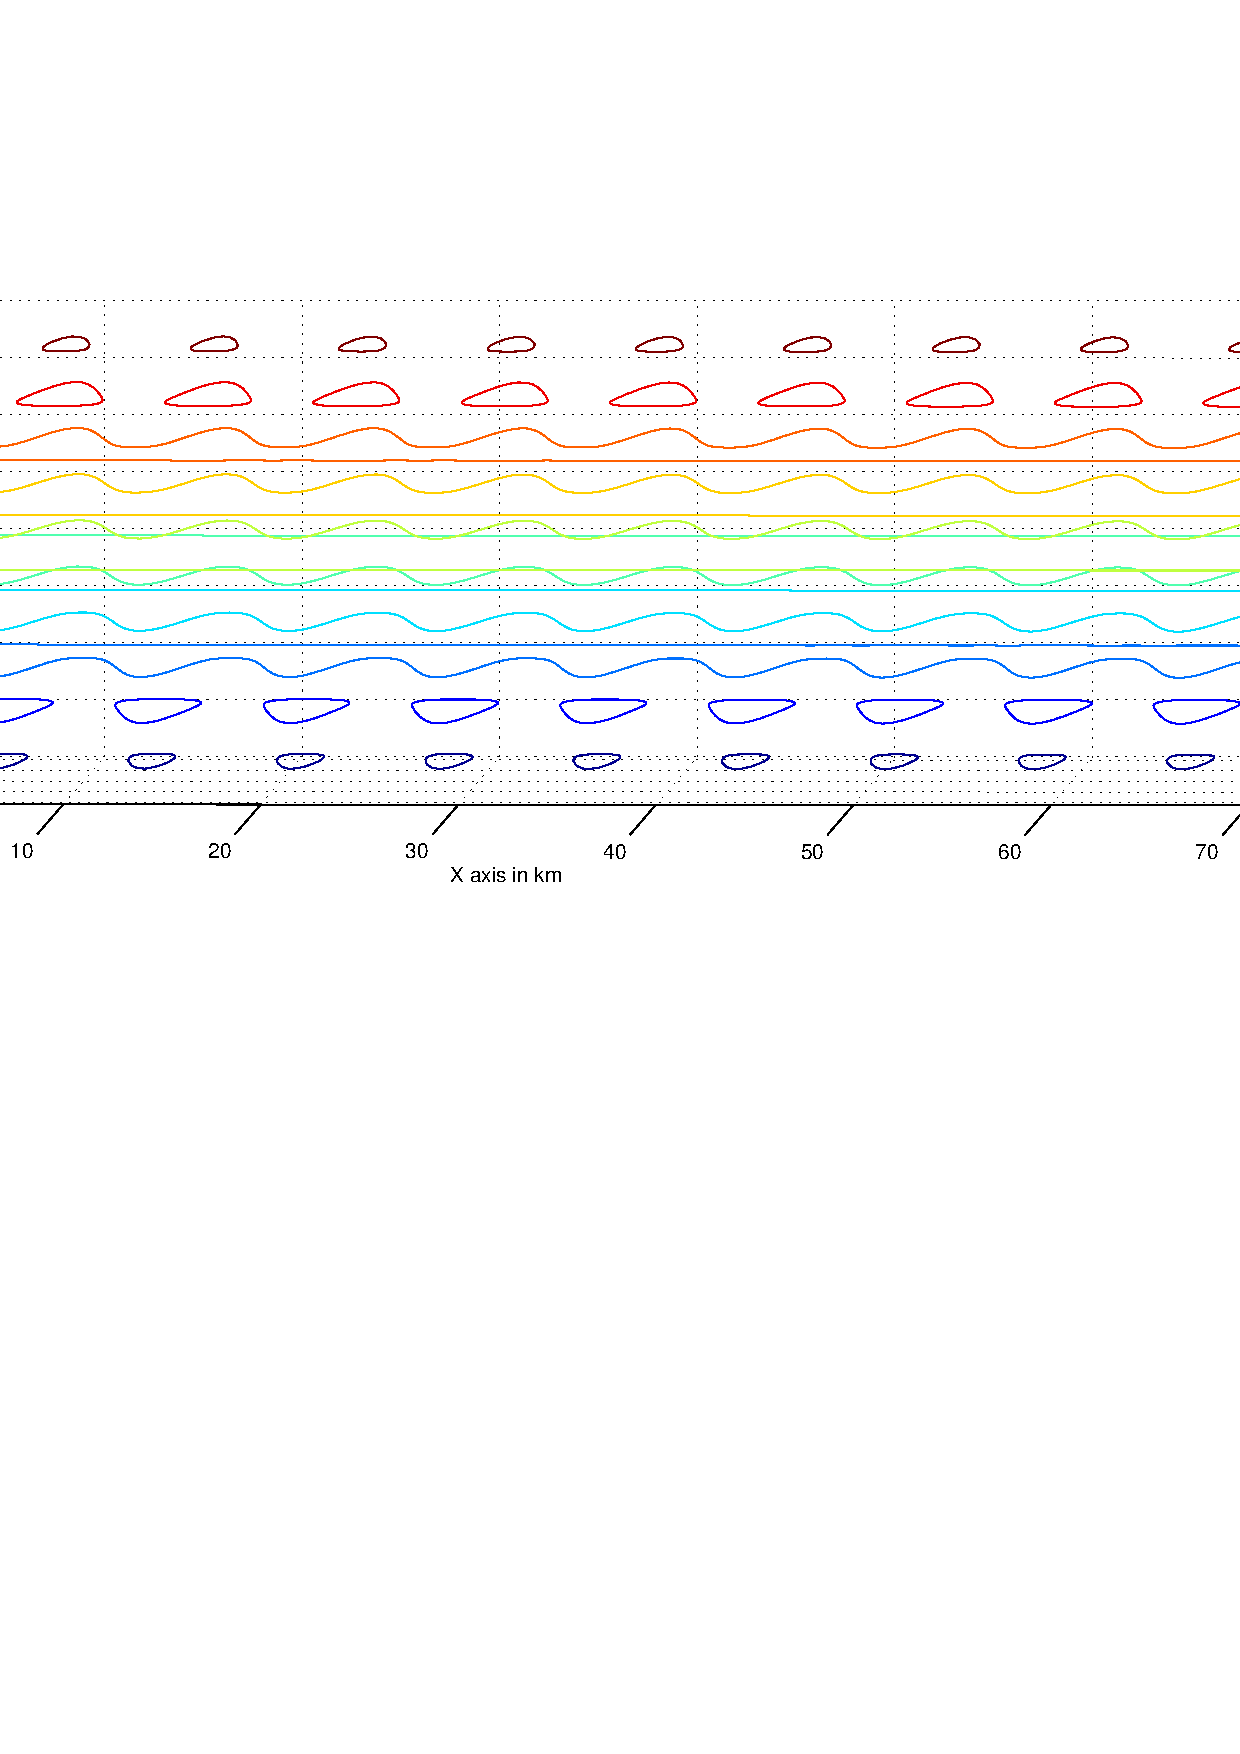
\includegraphics[width=2 in, height=1.5 in]{MCM.pdf}
% \vspace{-1em}
% \caption{ A plot of  \ref{eq:sf} at $t=0$.}
% \label{fig:kme}
% \end{minipage}
%\end{figure}
%\vspace{-1em}
%\begin{figure}[!htb]
%\begin{minipage}[]{.5\linewidth}
%\includegraphics[width=2 in, height=1 in]{start_end_50.pdf}
%\vspace{-1em}
% \caption{ Start and end points of 50 nodes}
%\label{fig:res11}
%\end{minipage}
%\begin{minipage}{.45\linewidth}
%\includegraphics[width=1 in, height=1 in,angle=-90]{points1.pdf}
%\vspace{-0.5em}
% \caption{probabilistic distribution}
%\label{fig:ges11}
% \end{minipage}
%\end{figure}
%\end{frame}
%%------------------------------------------------
%%\subsection{Problem Definition}
\begin{frame}
\frametitle{Problem Definition}
We define four probabilistic connectivity problem. They are 
\begin{itemize}
\item $\ACONN$ problem
\item $\ARCONN$ problem
\item $\SCONN$ problem
\item $\SRCONN$ problem
\end{itemize}
\end{frame}
%-----------------------------------------------
%-----------------------------------------------
\begin{frame}
\frametitle{the $\ACONN$ and $\ARCONN$ problems}
\begin{definition}[\textbf{the $A$-$CONN$ problem}]
\normalfont
Given a probabilistic network $G$ with no relay nodes, compute the probability $Conn(G)$ that the network is in a state where the sink node $s$ can reach all sensor nodes. 
\end{definition}

\begin{definition}[\textbf{the $AR$-$CONN$ problem}]
\normalfont
Given a probabilistic network $G$ where $V_{relay}$ is possibly non-empty, compute the probability $Conn(G)$ that the network is in a state where the sink node $s$ can reach all sensor nodes. 
\end{definition}

\end{frame}

%-----------------------------------------------
%-----------------------------------------------
\begin{frame}
\frametitle{the $\SCONN$ and $\SRCONN$ problems}

\begin{definition}[\textbf{the $S$-$CONN$ problem}]
Given a probabilistic network $G$ with no relay nodes, and a required number of sensor nodes $n_{req}\leq |V_{sense}|$, compute the probability $Conn(G,n_{req})$ that the network is in a state where the sink node $s$ can reach a subset of sensor nodes having at least $n_{req}$ sensor nodes. 
\end{definition}


\begin{definition}[\textbf{the $SR$-$CONN$ problem}]

Given a probabilistic network $G$ where $V_{relay}$ is possibly non-empty, and a required number of sensor nodes $n_{req}\leq |V_{sense}|$, compute the probability $Conn(G,n_{req})$ that the network is in a state where the sink node $s$ can reach a subset of sensor nodes having at least $n_{req}$ sensor nodes. 
\end{definition}

\end{frame}

%-----------------------------------------------

%-----------------------------------------------
%
%\begin{frame}
%\frametitle{Network State}
%\begin{itemize}
%\item A probabilistic graphs arises when network is in some particular network states.
%\item A state $S$ of $V$ can be specified by $\{v_1[i_1], v_2[i_2], . . . , v_n[i_n]\}$
%\item If locations are independent, we have $Pr(S) =\prod_{v_{\alpha}\in V} p_{v_\alpha[i_\alpha]}$.
%
%\item In the $A$-$CONN$ and $AR$-$CONN$ problem, a state is \textbf{operating} if the
%sink $s$ can reach all sensor nodes in $V_{sense}$ . 
%\item Similarly, in the $S$-$CONN$ and $SR$-$CONN$ problem, a state $S$ is \textbf{operating} if the sink node $s$ can reach a $n_{req}$ sensor
%nodes.
%\end{itemize}
%\vspace*{-0.5 cm}
%\begin{figure}[h]
%\centering
%\includegraphics[width=1.3 in, height=.8 in]{Figure1.pdf}
%\vspace*{-0.5 cm}
% \caption{ An example network}
%\end{figure}
%
%\end{frame}
%------------------------------------------------
%\subsection{Thesis Contribution}
\begin{frame}
\frametitle{Thesis Contribution}
Efficient dynamic programming algorithms
\begin{enumerate}
\item for the $\SRCONN$ problem on probabilistic networks whose underlying graphs are trees.% The algorithm solves the more restricted $\ARCONN$ problem with little overhead compared to a dedicated algorithm to solve the $\ARCONN$ problem.
\item for the $\ACONN$ problem on partial $k$-trees.
\item for the $\ARCONN$ and $\SRCONN$ problems on partial $k$-trees.
\end{enumerate}
All cases the algorithm runs in polynomial time for any fixed $k$. 
\end{frame}
%---------------
\section{$\ACONN$ problem}

\begin{frame}
\frametitle{Simulation Results for $\ACONN$ problem}

\begin{itemize}
\item Test Networks
\item Running Time
\item Connectivity for different partial $k$-trees
\end{itemize}
\end{frame}
%-----------------------------------------
\begin{frame}
\frametitle{Test Networks}
\begin{figure}[htbp]
\centering
\includegraphics[width=3.8 in, height=2 in]{NetworkI_paper.pdf}
\caption{$G_{10}$}
\end{figure}
\end{frame}
%-----------------------------------------
\begin{frame}
\frametitle{Test Networks(Cont.)}
\vspace{-0.7em}
\begin{figure}[htbp]
\centering
\includegraphics[width=3.8 in, height=1.2 in]{NetworkII.pdf}
\vspace{-1em}
\caption{$G_{12}$}
\end{figure}
\vspace{-1.5em}
\begin{figure}[htbp]
\centering
\includegraphics[width=3.8 in, height=1.5 in]{NetworkIII.pdf}
\vspace{-1em}
\caption{$G_{15}$}
\end{figure}
\end{frame}
%-----------------------------------------
\begin{frame}
\frametitle{Running Time}
\begin{table}[!htb]

    %\caption{Global caption}
    %\begin{minipage}{.5\linewidth}
   
      \centering
     \begin{tabular}{|c|c|c|c|}
     \hline
         k& Network $G_{10}$ & Network $G_{12}$ & Network $G_{15}$ \\
     \hline
     1&90& 130& 200 \\\hline
     2&1000 &1380&1480	\\\hline
3 &60000&875000&940000	 \\\hline
\end{tabular}
 \caption{Running time in milliseconds}
\label{Tab:runtym}
\end{table}

\end{frame}
%-----------------------------------------

%-----------------------------------------
\begin{frame}
\frametitle{Connectivity for different partial $k$-trees}
\begin{table}[!htb] 
      \centering
     \begin{tabular}{|c|c|c|c|}
     \hline
      k& Network $G_{10}$ & Network $G_{12}$ & Network $G_{15}$ \\
     \hline
      1 & 0.62&0.336& 0.82 \\\hline
2 &0.71 & 0.36& 0.99\\\hline
3 &0.75& 0.37& 1\\\hline
\end{tabular}
 \caption{Connectivity lower bounds using different partial $k$-trees}
 \label{Tab:acc}
\end{table}
\end{frame}
%-----------------------------------------
%%----------------------------------------
%-----------------------------------------
\section{$\ARCONN$ and $\SRCONN$ problems}
%%-----------------------------------------
%
%%\subsection{Algorithms for $\ARCONN$ and $\SRCONN$}
%%\subsection{Simulation Results for $\ARCONN$ and $\SRCONN$}
%\begin{frame}
%\frametitle{$\ARCONN$ and $\SRCONN$ problems}
%\begin{itemize}
%\item Simulation Results for $\ARCONN$ and $\SRCONN$ problems.
%\end{itemize}
%\end{frame}


%\begin{frame}
%\frametitle{$\ARCONN$ state types}
%
%\centerline{
%$AR\mbox{-}type(S)=\{V_{1,b(V_1)}^{Loc(V_1)}, V_{2,b(V_2)}^{Loc(V_2)}, \ldots, V^{Loc(V_r)}_{r,b(V_r)} \}$}
%\begin{example}
%\normalfont
%In figure \ref{fig:sttype1}, denote by $G_{v_i,1}$, the graph induced on nodes $\{v_a,v_b,v_i,v_j,v_k\}$. Assume that $\{v_b\}\in V_{sense}$ and $\{v_a,v_i,v_j,v_k\} \in V_{relay}$. Suppose that state $S$ of figure \ref{fig:sttype1_node} is a possible network state of $G_{v_i,1}$. Then $AR\mbox{-}type(S)=\big \{\{v_i\}_1^{(1)},\{v_j,v_k\}_0^{(2,3)}\big\}$. Here, the indicator $b(\{v_i\})=1$ since $v_b$ is a sensor node connected to $v_i$ in $S$. 
%\end{example}
%
%\begin{figure}[!htb]
%\begin{minipage}[]{0.45\linewidth}
%\includegraphics[width=1.5 in, height=1 in]{Ch5f2.pdf}
%\caption{A fragment of a 3-tree}
%\label{fig:sttype1}
%\end{minipage}
%\begin{minipage}{0.45\linewidth}
%\nwline
%\includegraphics[width=1.2 in, height=1 in]{Ch5f2_1.pdf}
%\caption{A state $S$ on $\{v_a,v_b,v_i,v_j,v_k\}$}
%\label{fig:sttype1_node}
%\end{minipage}
%\end{figure}
%\end{frame}
%%-----------------------------------------
%
%%-----------------------------------------
%\begin{frame}
%\frametitle{Merging State types}
%\begin{figure}
%\includegraphics[scale=0.8]{part.pdf}
%\caption{Merging two tables}
%\end{figure}
%\end{frame}
%%-----------------------------------------
%
%%-----------------------------------------
%\begin{frame}
%\frametitle{Removing Bad State Types}
%\begin{itemize}
%
%\item For the $\ARCONN$ problem, a state $S$ of the subgraph $G_{v_i,base}$ reduced onto the $k$-clique $K_{v_i,base}$.
%\item $S$ is considered bad if node $v_i$ appears as a singleton part and the indicator $b({v_i})=1$.
%\item The algorithm removes all such bad state types from $T_{v_i,base}$.
%
%\end{itemize}
%\end{frame}
%%-----------------------------------------

%-----------------------------------------
\begin{frame}
\frametitle{Simulation Results for $\ARCONN$ and $\SRCONN$ problems}
\begin{itemize}
\item Test Networks
\item Running time
\item Effects of Adding Relay nodes
\end{itemize}
\end{frame}
%-----------------------------------------

%-----------------------------------------
\begin{frame}
\frametitle{Test Networks}
\vspace{-0.5em}
\begin{figure}[!htb]
\begin{minipage}{.8\linewidth}
\includegraphics[width=4 in, height=1.2 in]{NetworkI_paper.pdf}
\caption{Network $G_{10}$}
\label{fig:netI1}
\end{minipage}
\begin{minipage}{.8\linewidth}
\includegraphics[width=4 in, height=1.2 in]{NetworkI_paper_Relay.pdf}
\vspace{-0.7 cm}
\caption{Network $G_{10,3}$}
\label{fig:netIR}
\end{minipage}
\end{figure}

\end{frame}
%-----------------------------------------

%-----------------------------------------
\begin{frame}
\frametitle{Running Time}
\begin{table}[!htb]
    %\caption{Global caption}
    \begin{minipage}{1\linewidth}
   
      \centering
     \begin{tabular}{|c|c|c|}
     \hline
         k& Network $G_{10}$ &Network $G_{10,3}$\\
     \hline
     1&90& 110 \\\hline
     2&1000 &6000	\\\hline
3 &6000&8000	 \\\hline
\end{tabular}
 \caption{Running time in milliseconds}
\label{Tab:rtym1}
    \end{minipage}
\end{table}

\end{frame}
%-----------------------------------------

%-----------------------------------------
\begin{frame}
\frametitle{Effect of adding relay nodes}

\begin{table}[!htb]
  \centering
 \begin{minipage}{.5\linewidth}
     \begin{tabular}{|c|c|c|}
     \hline
     k & Network $G_{10}$ & Network $G_{10,3}$  \\
     \hline
      1 & 0.30 & 0.86 \\\hline
	  2 & 0.54 & 0.96\\\hline
	  3 &0.60 & 0.98 \\\hline
\end{tabular}
    \end{minipage}
     \caption{Connectivity with respect to $k$}
      \label{Tab:SRC}   
\end{table}
\end{frame}
%-----------------------------------------

%-----------------------------------------
\begin{frame}
\frametitle{Effect of adding relay nodes for various node $R_{tr}$:}

\begin{figure}[!htb]
\begin{minipage}{.9\linewidth}
\end{minipage}
\includegraphics[width=4 in, height=1.75 in]{NetworkI_woR-eps-converted-to.pdf}
\caption{Connectivity versus transmission range}
\label{Fig:NWOR}
\end{figure}

\end{frame}
%--------------
%\begin{frame}
%\frametitle{The $\SRCONN$ State Types}
%
%
%\centerline{
%$SR\mbox{-}type(S)=\{V_{1,c(V_1)}^{Loc(V_1)}, V_{2,c(V_2}^{Loc(V_2)}, \ldots, V^{Loc(V_r)}_{r,c(V_r} \}$}
%
%\begin{example}
%\normalfont
% In figure \ref{fig:sttype2}, denote by  $G_{v_i,1}$, the graph induced on nodes $\{v_a,v_b,v_i,v_j,v_k\}$. Assume that $\{v_b,v_i\}\in V_{sense}$ and $\{v_a,v_j,v_k\} \in V_{relay}$. Suppose that state $S$ of figure \ref{fig:sttype2_node} is a possible network state of $G_{v_i,1}$. Then $SR\mbox{-}type(S)=\big \{\{v_i\}_2^{(1)},\{v_j,v_k\}_0^{(2,3)}\big\}$. Here, the count $c(\{v_i\})=2$ since both of $v_i$ and $v_b$ are sensor nodes.
% 
%\end{example}
%\vspace*{-0.4 cm}
%\begin{figure}[!htb]
%\begin{minipage}[]{0.45\linewidth}
%\includegraphics[width=1.5 in, height=1 in]{Ch5f3.pdf}
%\caption{A 3-tree fragment}
%\label{fig:sttype2}
%\end{minipage}
%\begin{minipage}{0.45\linewidth}
%\includegraphics[width=1.2 in, height=1 in]{Ch5f3_1.pdf}
%\caption{A state $S$ on $\{v_a,v_b,v_i,v_j,v_k\}$}
%\label{fig:sttype2_node}
%\end{minipage}
%\end{figure}
%
%\end{frame}
%%-----------------------------------------
%%--------------
%\begin{frame}
%\frametitle{Merging State types}
%\begin{figure}
%\includegraphics[scale=0.8]{partition1.pdf}
%\caption{Merging two tables}
%\end{figure}
%\end{frame}
%%-----------------------------------------
%%--------------
%\begin{frame}
%\frametitle{Bad State Types}
%\begin{itemize}
%
%\item For the $\SRCONN$ problem, a state $S$ of the subgraph $G_{v_i,base}$ reduced onto the $k$-clique $K_{v_i,base}$.
%\item $S$ is considered bad if node $v_i$ appears as a singleton part and the indicator $c({v_i})\geq 1$.
%\item The algorithm removes all such bad state types from $T_{v_i,base}$.
%
%\end{itemize}
%\end{frame}
%-----------------------------------------
\begin{frame}
\frametitle{$\SRCONN$ Simulation Results}
A designer has at least 3 options to achieve a minimum required $Conn(G,n_{req})$ value:

\begin{itemize}
\item tuning the $n_{req}$ parameter,
\item tuning node transmission range $R_{tr}$, and
\item tuning the number of deployed relay nodes.
\end{itemize}
\end{frame}


\begin{frame}
\frametitle{Effect of varying $n_{req}$} 
\begin{itemize}
\item Figure \ref{Fig:CvCwr1} illustrates the achieved $Conn(G,n_{req})$ as $n_{req}$ varies in the range $[1,10]$.
\item Figure \ref{Fig:CvCwr2} illustrates the achieved $Conn(G,n_{req})$ as $n_{req}$ varies in the range $[1,10]$, and $R_{tr}$ varies in the range $[2.5,5.5]$.

\end{itemize}
\begin{figure}[!htb]
\begin{minipage}{0.5\linewidth}
\centering
\includegraphics[width=2 in, height=1.5 in]{abc.pdf}
\caption{Connectivity versus $n_{req}$}
\label{Fig:CvCwr1}
\end{minipage}
\begin{minipage}{0.45\linewidth}
\centering
\includegraphics[width=2 in, height=1.5 in]{3D.pdf}
\caption{Connectivity versus $n_{req}$ and transmission range}
\label{Fig:CvCwr2}
\end{minipage}
\end{figure}

\end{frame}
%-----------------------------------------
%-----------------------------------------
\begin{frame}
\frametitle{Concluding Remarks}
\begin{itemize}
\item This thesis is motivated by recent interest in UWSNs as a platform for preforming many useful tasks. 
\item A challenge arises since sensor nodes incur small scale and large scale movements that can disrupt network connectivity.
\item  Thus, tools for quantifying the likelihood that a network remains completely or partially connected become of interest.

\item To this end, the thesis has formalized 4 probabilistic connectivity problems, denoted $\ACONN,$ $ \SCONN, \ARCONN, \mbox{ and } \SRCONN$. 
\item The obtained results show that all of the 4 problems admit polynomial time algorithms on $k$-trees (and their subgraph), for any fixed $k$.
\item  The running time of the algorithms, however, increase exponentially as $k$ increases. Thus, more work needs to be done towards obtaining more effective algorithms.
\end{itemize}
\end{frame}
%-----------------------------------------
\section{Future Research Directions}
\begin{frame}
\frametitle{Future Research Directions}
\begin{itemize}
\item Investigating the applicability of our algorithm to some other classes of graph to be a worthwhile direction.

\item It is interesting to analyze the delays incurred in typical data collection rounds.
\item It is worthwhile to investigate area coverage assuming a probabilistic locality model of the nodes.
\end{itemize}

\end{frame}
%-----------------------------------------


%-----------------------------------------
\begin{frame}
\frametitle{}
\begin{center}
\Huge Thanks!
\end{center}

\end{frame}
%-----------------------------------------
\end{document} 